% This text is proprietary.
% It's a part of presentation made by myself.
% It may not used commercial.
% The noncommercial use such as private and study is free
% Sep. 2005 
% Author: Sascha Frank 
% University Freiburg 
% www.informatik.uni-freiburg.de/~frank/
%
% additional usepackage{beamerthemeshadow} is used
%  
%  \beamersetuncovermixins{\opaqueness<1>{25}}{\opaqueness<2->{15}}
%  with this the elements which were coming soon were only hinted
%\documentclass[8pt]{beamer}
\documentclass[10pt]{beamer}
\usepackage{etex}
\newenvironment<>{varblock}[2][\textwidth]{%
  \setlength{\textwidth}{#1}
  \begin{actionenv}#3%
    \def\insertblocktitle{#2}%
    \par%
    \usebeamertemplate{block begin}}
  {\par%
    \usebeamertemplate{block end}%
  \end{actionenv}}
%\usepackage{hyperref}
%\usepackage{natbib}
%\usepackage{beamerthemeshadow}
\usepackage{beamerinnerthemecircles, beamerouterthemeshadow}

\usepackage{amsmath,amssymb,amsfonts}
\usepackage[pdf]{pstricks}
%\usepackage{bbm}
%\usepackage{booktabs}
\usepackage{amsthm}
\usepackage{booktabs}
\usepackage{graphicx}
\usepackage{epsfig}
%\usepackage{graphics}

% MQ: This is to be able to compile on the Riksbank computer. Uncomment with my laptop. Ugly solution but will have to do for now.
%\usepackage{epstopdf}
%\epstopdfsetup{outdir=./}

\usepackage{rotating}

\usepackage{url}
\usepackage{breqn}
%\usepackage{hyperref}
\usepackage[authoryear]{natbib}
\usepackage{setspace}
\usepackage{multirow}
%\usepackage{harvard}
\usepackage{xcolor}
%\usepackage{multicolumn}
\usepackage{algpseudocode}
\usepackage{sidecap}
\usepackage{bbm} 
\usepackage{courier}
\usepackage{tikz}
\usetikzlibrary{arrows,shapes,snakes,automata,backgrounds,petri}

\tikzset{
  treenode/.style = {align=center, inner sep=0pt, text centered,
    font=\sffamily},
  arn_n/.style = {treenode, circle, white, font=\sffamily\bfseries, draw=black,
    fill=black, text width=1.5em},% arbre rouge noir, noeud noir
  arn_r/.style = {treenode, circle, red, draw=red, 
    text width=1.5em, very thick},% arbre rouge noir, noeud rouge
  arn_x/.style = {treenode, rectangle, draw=black,
    minimum width=0.5em, minimum height=0.5em}% arbre rouge noir, nil
}
\beamertemplatenavigationsymbolsempty

\newenvironment{myenumerate}{\begin{enumerate}[(1)]}{\end{enumerate}} 
\sidecaptionvpos{figure}{c}
% FOR COLORING PARTS  OF TABLE
%\usepackage[beamer,customcolors]{hf-tikz}

%\tikzset{hl/.style={
%    set fill color=red!80!black!40,
%    set border color=red!80!black,
%  },
%}

\mode<presentation> {
    \usetheme{Madrid} %Frankfurt} %Bergen, Berkely, Berlin, Boadilla, CambridgeUS, Darmstadt,
                          %Frankfurt, Goettingen, Singapore, Warsaw
    \usecolortheme{beaver} %seahorse} %default} %beetle, seahorse, wolverine, dolphin, beaver
    %\useoutertheme[subsection=true]{smoothbars} 
    \usefonttheme{default}
    %\usecolortheme{red}
    

	\setbeamercolor{block title}{use=unstructure, fg=white, bg=purple!75!black} %{use=structure,fg=white,bg=purple!75!black}
	%\setbeamercolor{block body}{use=structure,fg=black,bg=white!20!white}    
    %\setbeamercolor{block body}{bg=white}
    \setbeamertemplate{enumerate items}[default]
    \setbeamercolor{enumerate item}{fg=purple!75!black} 
    \setbeamercolor{enumerate subitem}{fg=purple!75!black} 	 
	\setbeamercolor{itemize item}{fg=purple!75!black}  
	\setbeamertemplate{itemize item}[triangle]  
	\setbeamercolor{itemize subitem}{fg=purple!75!black}
	\setbeamertemplate{itemize subitem}[triangle]
	\setbeamertemplate{blocks}[framed]


}



%\usepackage{colortbl}
%\definecolor{yellow}{cmyk}{0,0.18,0.90,0.00}

%\usepackage{xcolor}

%\usepackage[authoryear]{natbib}
\begin{document}
\title[Lecture 9]{Bayesian Learning 732A46: Lecture 9}  
\author[Matias Quiroz]{Matias Quiroz\inst{1}$^{,}$\inst{2}}
\setbeamerfont{institute}{size=\fontsize{7pt}{8pt}}
\institute[LiU and Riksbank]{
  \inst{1}%
   Division of Statistics and Machine Learning, Link\"{o}ping University\\~\\
  \inst{2}%
   Research Division, Sveriges Riksbank\\
     
}

%\institute[Riksbank and LiU]{Sveriges Riksbank and Division of Statistics and Machine Learning, Link\"{o}ping University}

\date[]{May 2016} %\today 

%\usebackgroundtemplate{%
%  \vbox to \paperheight{\vfil\hbox to \paperwidth{\hfil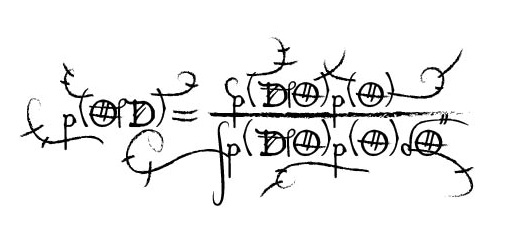
\includegraphics[width=1.5in]{Bayes.jpg}\hfil}\vfil}
%}

{
%\usebackgroundtemplate{\begin{center}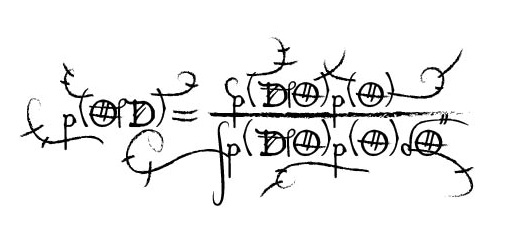
\includegraphics[width=0.4\paperwidth]{Bayes.jpg}\end{center}}
\usebackgroundtemplate{%
  \vbox to \paperheight{\hbox to \paperwidth{\hfil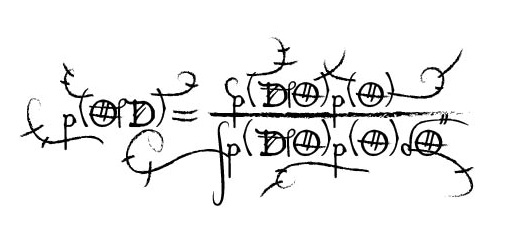
\includegraphics[width=2in]{Bayes.jpg}\hfil}}
}
\begin{frame}
\titlepage
\end{frame}
}
%\frame{\titlepage} 

%\frame{\frametitle{Overview of the talk}\tableofcontents}


\begin{frame}
\frametitle{Lecture overview}

\begin{itemize}
\item The Metropolis sampler
\bigskip
\item The Metropolis-Hastings sampler 
\bigskip
\item Metropolis-Hastings within Gibbs sampler
\bigskip
\item Why does MCMC work?
\bigskip
\item Measures of efficiency
\bigskip
\item Assessing converge of MCMC simulation

\end{itemize}

\end{frame}

\begin{frame}
\frametitle{The general idea from last week}
\begin{itemize}
\item Construct a \textbf{Markov sequence} with the property
$$\{\theta^{(i)}\}_{i\geq J}^N\text{ is distributed according to } \pi(\theta) \textbf{ for large enough }J.$$
\medskip
\item The posterior $\pi(\theta)$ is the \textbf{\color{blue}stationary distribution} of the Markov chain.
\medskip
\item The period $0,1,\dots J$ is the \textbf{\color{blue}burn-in period} of the chain. 
\medskip
\item The draws obtained are used for computing the \textbf{expectation of a function}. \textbf{\color{blue}Average a function over the posterior distribution}.
\medskip
\item Even if the draws are dependent, still true that
$$\frac{1}{N}\sum_{i=1}^N h(\theta^{(i)}) \xrightarrow{a.s} E[h(\theta)]=\int h(\theta)\pi(\theta)d\theta.$$
\end{itemize}

\end{frame}




\begin{frame}
\frametitle{The Metropolis algorithm}
\begin{itemize}
\item \textbf{\color{blue}Powerful} when distributions are \textbf{\color{red}not of known form}, not even after conditioning.\bigskip
\item A \textbf{\color{blue}Markov chain version} of \textbf{rejection sampling}. \bigskip
\item \textbf{\color{blue}Only requirement}: $\pi(\theta)$ can be \textbf{evaluated} (up to $\propto$) \bigskip
\item The \textbf{\color{blue}Metropolis} requires a symmetric proposal distribution.\bigskip
\item \textbf{\color{blue}Metropolis-Hastings}: \textbf{relaxes} the symmetry requirement.
\end{itemize}

\end{frame}


\begin{frame}
\frametitle{The Metropolis algorithm}
\begin{center}
\begin{minipage}{\columnwidth}
\begin{varblock}[1\columnwidth]{The Metropolis algorithm}
Obtain $N$ samples from $\pi(\theta)\propto p(y|\theta)p(\theta)$.
\begin{itemize}
\item Set an (arbitrary) start point $$\theta_c = \theta^{(0)},$$
where $\theta_c$ denotes \textbf{\color{blue}the current state} of the chain.
\item \textbf{For} $i=1,\dots, N$, \textbf{repeat}
\end{itemize}
\begin{enumerate}
\item \textbf{Propose} a draw $\theta_p \sim q(\theta | \theta_c)$ ($q$ - {\color{blue}proposal distribution}).
\item Evaluate $$\alpha(\theta_c, \theta_p) = \min \left(1, \frac{\pi(\theta_p)}{\pi(\theta_c)} \right) = \min \left( 1, \frac{p(y|\theta_p)p(\theta_p)}{p(y|\theta_c)p(\theta_c)} \right) .$$
\item Sample $u\sim \textrm{uniform}(0,1)$.
\item {\color{blue}If} $u\leq \alpha(\theta_c, \theta_p) \implies \theta^{(i)}=\theta_p$, {\color{blue}else}  $\theta^{(i)}=\theta_c$
\end{enumerate}
\end{varblock}
\end{minipage}
\end{center}

\end{frame}


\begin{frame}
\frametitle{The Metropolis algorithm, cont}
\begin{itemize}
\item \textbf{\color{blue}"Climbing up the hill"} will always be accepted. 
\medskip
\item \textbf{\color{blue}"Down the hill"} accepted with fraction $\pi(\theta_p)/\pi(\theta_c)$. 
\medskip
\item \textbf{\color{red}Note}: if we reject the draw we \textbf{keep the current draw in the chain}. A Metropolis that rejects \textbf{too often} gives a "sticky" chain.
\medskip
\item \textbf{\color{blue}Common choice of proposal}: $q(\cdot|\theta_c) = \mathcal{N}(\theta_c, \Sigma)$ (has to be symmetric). \textbf{\color{blue}Random walk} type (notice the mean).
\medskip
\item $\Sigma = \tilde{c}I$. Choose $\tilde{c}$ so that your \textbf{\color{blue}acceptance probability} (on average) is $\alpha\approx 0.23$. 
\medskip
\item If the parameters are \textbf{\color{red}heavily correlated}: $\Sigma = \tilde{c} \Sigma_{\theta^{\star}}$, where $\Sigma_{\theta^\star}$ is the \textbf{posterior covariance} evaluated at the mode $\theta^{\star}$ (\textbf{\color{blue}recall}: \texttt{optim} in \texttt{R}).
\medskip
\item \textbf{Question:} Why do you think that $\alpha \approx 1$ is \textbf{\color{red}not} desirable with a Random walk proposal?
\pause
\item Will give a \textbf{\color{blue}slow mixing} (\textbf{inefficient}) chain. More on this later.
\end{itemize}
\end{frame}

%\frame{\frametitle{Example: Logistic regression revisited.}
%\begin{itemize}
%\item[4.] \textbf{R-script} \texttt{logitRWMetropolis.R}: Simulates from the model and computes the posterior by \textbf{\color{blue}Random Walk Metropolis sampling}.
%
%\begin{figure}[H]
%%\includegraphics[width=0.7\columnwidth]{RejectionSampling}
%%\protect\caption{$\p(\alpha, \beta|y)$}
%\end{figure}
%\item \textbf{Homework:} Play with the code. \textbf{Make sure you understand} how to code the posterior {\color{blue}in logarithmic scale}. \textbf{\color{red}Extra:} Modify the code to handle more regressors (parameters). How many parameters are feasible?
%\item If you did the \textbf{\color{red}extra} from Lecture 2, can you handle more parameters now? (\textbf{\color{blue}you should}!)
%\end{itemize}
%}


\begin{frame}
\frametitle{The Metropolis-Hastings algorithm}
\begin{itemize}
\item A \textbf{more general} version of the \textbf{\color{blue}Metropolis algorithm}.
\medskip
\item \textbf{\color{blue}Same setting}: we can evaluate $$\pi(\theta) \propto p(y|\theta)p(\theta).$$
\medskip
\item \textbf{\color{blue}Metropolis-Hastings}: Symmetry of proposal is not required. 
\medskip
\item \textbf{\color{red}What do we gain?}: can move away from a \textbf{Random Walk} (RW) $q()$. 
\medskip
\item \textbf{Note}: 
\\ The RW proposal is \textbf{\color{blue}local} (proposes from the \textbf{\color{red}current state} of the chain). \textbf{\color{blue}Moves around slowly} in $\theta$ space.
\medskip
\item A \textbf{good proposal} $q()$ explores the parameter space \textbf{efficiently}.
\\ \textbf{\color{blue}Propose globally} (where the posterior mass is located). 

\end{itemize}

\end{frame}


\begin{frame}
\frametitle{The Metropolis-Hastings algorithm, cont.}
\begin{center}
\begin{minipage}{\columnwidth}
\begin{varblock}[1\columnwidth]{The Metropolis-Hastings algorithm}
Obtain $N$ samples from $\pi(\theta)\propto p(y|\theta)p(\theta)$.
\begin{itemize}
\item Set an (arbitrary) start point $$\theta_c = \theta^{(0)},$$
where $\theta_c$ denotes \textbf{\color{blue}the current state} of the chain.
\item \textbf{For} $i=1,\dots, N$, \textbf{repeat}
\end{itemize}
\begin{enumerate}
\item \textbf{Propose} a draw $\theta_p \sim q(\theta | \theta_c)$ ($q$ - {\color{blue}proposal distribution}).
\item Evaluate $$\alpha(\theta_c, \theta_p) = \min \left(1, \frac{\pi(\theta_p)/q(\theta_p | \theta_c)}{\pi(\theta_c)/q(\theta_c | \theta_p)} \right) = \min \left( 1, \frac{p(y|\theta_p)p(\theta_p)/q(\theta_p | \theta_c)}{p(y|\theta_c)p(\theta_c)/q(\theta_c | \theta_p)} \right) .$$
\item Sample $u\sim \mathrm{uniform}(0,1)$.
\item {\color{blue}If} $u\leq \alpha(\theta_c, \theta_p) \implies \theta^{(i)}=\theta_p$, {\color{blue}else}  $\theta^{(i)}=\theta_c$
\end{enumerate}
\end{varblock}
\end{minipage}
\end{center}

\end{frame}

\begin{frame}
\frametitle{The Metropolis-Hastings algorithm, cont}
\begin{itemize}
\item \textbf{\color{blue}Note}: if $q(\theta)=\text{symmetric} \implies$ \textbf{\color{blue}Metropolis} algorithm [$q$ cancels].
\item \textbf{\color{blue}Independence Metropolis-Hastings}:
$$q(\theta | \theta_c) = q(\theta) \quad \text{[ind. of the current state (\textbf{\color{red}not a RW})]}$$
\item \textbf{Example}: $$q(\cdot)=t_{\nu}(\theta^{\star}, \Sigma_{\theta^{\star}}),$$
where
\begin{eqnarray*}
\theta^{\star} & = & \text{the {\textbf{\color{blue}mode}} from a numerical optimization} \\
\Sigma_{\theta^{\star}} & = & \text{the {\textbf{\color{blue}covariance}} at } \theta^{\star} \quad [-H_{\theta^{\star}}^{-1}].
%$\theta^{*}$ & $=$ & 1 \\
\end{eqnarray*}
\item Very efficient... \textbf{but can get stuck}!
\item Make sure $t_{\nu}(\theta^{\star}, \Sigma_{\theta^{\star}})$ has \textbf{\color{red}heavier tails} than $p(y|\theta)p(\theta)$. 
 
\end{itemize}
\end{frame}

\begin{frame}
\frametitle{Metropolis-Hastings within Gibbs algorithm}
\begin{itemize}
\item \textbf{\color{blue}Recall Gibbs}: sample the \textbf{blocks} $\theta = (\theta_1, \dots, \theta_K).$, by
$$\pi(\theta_1|\theta_2, \theta_3 \dots, \theta_K)$$
$$\vdots$$
$$\pi(\theta_K|\theta_1, \theta_2, \dots, \theta_{K-1})$$
\item \textbf{Assumption}: can sample from each \textbf{full conditional} [\textbf{\color{blue}known form}].
\item \textbf{What if} not all are of known form? \textbf{\color{blue}M-H within Gibbs} to the rescue.
\item \textbf{\color{blue}Example:} let $K=3$ and suppose $\pi(\theta_2|\theta_1, \theta_3)$ is \textbf{\color{red}not} of known form.
\item[] Updating $\theta_2$ \textbf{at iteration} $i$: \textbf{\color{blue}Propose}
$$\theta_p = \theta_2^{(i)} \sim q(\theta_2 | \theta_1^{(i)}, \theta_2^{(i-1)}, \theta_3^{(i-1)})\quad \left[\textbf{\color{blue}Note}: \theta_c = \theta_2^{(i-1)}\right].$$
\item[] Then $$\alpha=\min \left( 1, \frac{\pi(\theta_p|\theta_1^{(i)},\theta_3^{(i-1)})/q(\theta_p | \theta_1^{(i)}, \theta_c, \theta_3^{(i-1)})}{\pi(\theta_c|\theta_1^{(i)},\theta_3^{(i-1)})/q(\theta_c| \theta_1^{(i)}, \theta_p, \theta_3^{(i-1)})} \right), \text{ \textbf{decide} to accept/reject}.$$
\end{itemize}
\end{frame}

\begin{frame}{Heteroscedastic regression}



\begin{itemize}
\item \textbf{\textcolor{blue}{M-H within Gibbs: Heteroscedastic regression}}:
\[
y_{i}=x_{i}'\beta+\varepsilon_{i}
\]
where the errors are \textbf{\color{red}heteroscedastic} 
\[
\varepsilon_{i}\sim \mathcal{N}\left(0,\sigma^{2}\exp\left(x_{i}'\gamma\right)\right).
\]
%\medskip{}

\item \textbf{\color{blue}Priors}: 
\begin{itemize}
\item \textbf{Multivariate normal} for $\beta$ and $\gamma$. 
\item Inv-$\chi^{2}$ for $\sigma^{2}$. %\medskip{}
\end{itemize}
\medskip

\item \textbf{\textcolor{blue}{Gibbs sampling} (two blocks)}:

\begin{itemize}
\item $\beta,\sigma^{2}\vert \gamma,y$
\medskip
\item $\gamma\vert\beta,\sigma^{2},y$
\end{itemize}
\end{itemize}
\end{frame}

\begin{frame}{M-H within Gibbs: Heteroscedastic regression, cont.}

\begin{itemize}
\item Draws from $\beta,\sigma^{2}\vert\gamma,y$ can be obtained as in standard (\textbf{homoscedastic}) linear regression but on \textbf{\color{blue}transformed data}. \textbf{Standard trick}.
\medskip
\item Rewrite the model as
\[
\tilde{y}_{i}=\tilde{x}_{i}'\beta+\tilde{\varepsilon}_{i},
\]
where 
\begin{itemize}
\item $\tilde{y}_{i}=\exp\left(-x_{i}'\gamma/2\right)y_{i}$
\item $\tilde{x}_{i}'=\exp\left(-x_{i}'\gamma/2\right)x_{i}'$
\item $\tilde{\varepsilon}_{i}=\exp\left(-x_{i}'\gamma/2\right)\varepsilon_{i}$. 
\item Note that $Var(\tilde{\varepsilon}_{i})=\sigma^{2}$, so \textbf{\color{blue}homoscedastic}. 
\end{itemize}\medskip
\item $p(\beta,\sigma^{2}\vert\gamma , y)$ - using a $\mathcal{N}\text{-Inv-}\chi^2$ conjugate prior ({\color{red}with transformed data}).\medskip
\item $p(\gamma\vert\beta,\sigma^{2},y)$ is non-standard,
but we can use \textbf{M-H to sample} with a Random walk proposal...\medskip
\item ... Or an \textbf{\color{blue}independence M-H proposal} $\mathcal{N}(\gamma^{\star},\Sigma_{\gamma^{\star}})$, $\gamma^{\star},\Sigma_{\gamma^{\star}}$ obtained with \texttt{optim} in \texttt{R}.
\end{itemize}
\end{frame}


\begin{frame}
\frametitle{Connecting the Gibbs sampler to M-H}
\begin{itemize}
\item \textbf{Updating a block} in a \textbf{Gibbs} step is a \textbf{\color{blue}special case} of M-H where $$\textbf{\color{red}Proposal} = \textbf{\color{red}Full conditional posterior},$$
so that $\alpha=1$.
\item \textbf{In our example}
$$q(\theta_2 | \theta_1^{(i)}, \theta_2^{(i-1)}, \theta_3^{(i-1)}) = \pi(\theta_2|\theta_1^{(i)},\theta_3^{(i-1)}) \quad \left[\textbf{\color{blue}gives }\alpha = 1\right].$$
\end{itemize}
\end{frame}

\begin{frame}
\frametitle{Why does MCMC work?}
\begin{itemize}
\item \textbf{\color{blue}Excellent paper}: Chib and Greenberg (1995).
\item The \textbf{transition kernel} of the M-H Markov chain:
$$T(\theta_c \rightarrow d\theta_p) = \overbrace{\int T(\theta_c \rightarrow \theta_p)d\theta_p}^{{\color{blue}\Pr(\text{move})}} + \overbrace{r(\theta_c)}^{{\color{blue}\Pr(\text{stay})}}\delta_{\theta_c}(d\theta_p),$$
\textbf{where}
$$T(\theta_c \rightarrow \theta_p)=q(\theta_p|\theta_c)\alpha(\theta_c,\theta_p)\quad \text{and } r(\theta_c)=1-\int T(\theta_c \rightarrow \theta_p)d\theta_p,$$
\textbf{with} $$\delta_{\theta_c}(d\theta_p)=\begin{cases} 1, \quad \text{if }\theta_c \in d\theta_p \\ 0, \quad \text{if }\theta_c \notin d\theta_p. \end{cases}$$
\item \textbf{\color{blue}M-H} chooses $\alpha$ so that 
$$\pi(\theta_c)T(\theta_c \rightarrow \theta_p)=\pi(\theta_p)T(\theta_p \rightarrow \theta_c)\quad  [\textbf{\color{blue}detailed balance}].$$
\end{itemize}
\end{frame}

\begin{frame}
\frametitle{Why does MCMC work?, cont.}
\begin{itemize}
\begin{proof}[\small{Proof that M-H's transition kernel fulfills \textbf{\color{yellow}detailed balance} [extra, if you are interested]}]
\small{$$\left[\alpha(\theta_c, \theta_p) = \min \left(1, \frac{\pi(\theta_p)/q(\theta_p | \theta_c)}{\pi(\theta_c)/q(\theta_c | \theta_p)} \right) \quad \text{and} \quad T(\theta_c \rightarrow \theta_p) = q(\theta_p | \theta_c)\alpha(\theta_c, \theta_p)\right]$$}
\vspace{-5mm}
{\small
\begin{eqnarray*}
\pi(\theta_c)T(\theta_c \rightarrow \theta_p)  &= & \pi(\theta_c)q(\theta_p | \theta_c)\min \left(1, \frac{\pi(\theta_p)/q(\theta_p | \theta_c)}{\pi(\theta_c)/q(\theta_c | \theta_p)} \right) \\
 & = & \pi(\theta_c)q(\theta_p | \theta_c)\min \left(\frac{\pi(\theta_c)q(\theta_p | \theta_c)}{\pi(\theta_c)q(\theta_p | \theta_c)}, \frac{\pi(\theta_p)q(\theta_c | \theta_p )}{\pi(\theta_c)q(\theta_p | \theta_c)} \right) \\
  & = & \pi(\theta_p)q(\theta_c | \theta_p ) \min \left(\frac{\pi(\theta_c)q(\theta_p | \theta_c)}{\pi(\theta_p)q(\theta_c | \theta_p )}, 1  \right) \\
  & = & \pi(\theta_p)q(\theta_c | \theta_p )\alpha(\theta_p, \theta_c) \\
& = & \pi(\theta_p)T(\theta_p \rightarrow \theta_c).
\end{eqnarray*}
Thus, $\pi(\theta)$ is the \textbf{\color{blue}stationary distribution} of the Markov chain generated by \textbf{\color{blue}M-H}. 

}
\end{proof}
\item \textbf{\color{blue}Convergence to} $\pi(\theta)$: $q$ has \textbf{\color{red}positive density} on the support of $\pi(\theta)$.  
\end{itemize}
\end{frame}


\begin{frame}
\frametitle{Illustrating the concept of efficiency}
\begin{figure}[H]
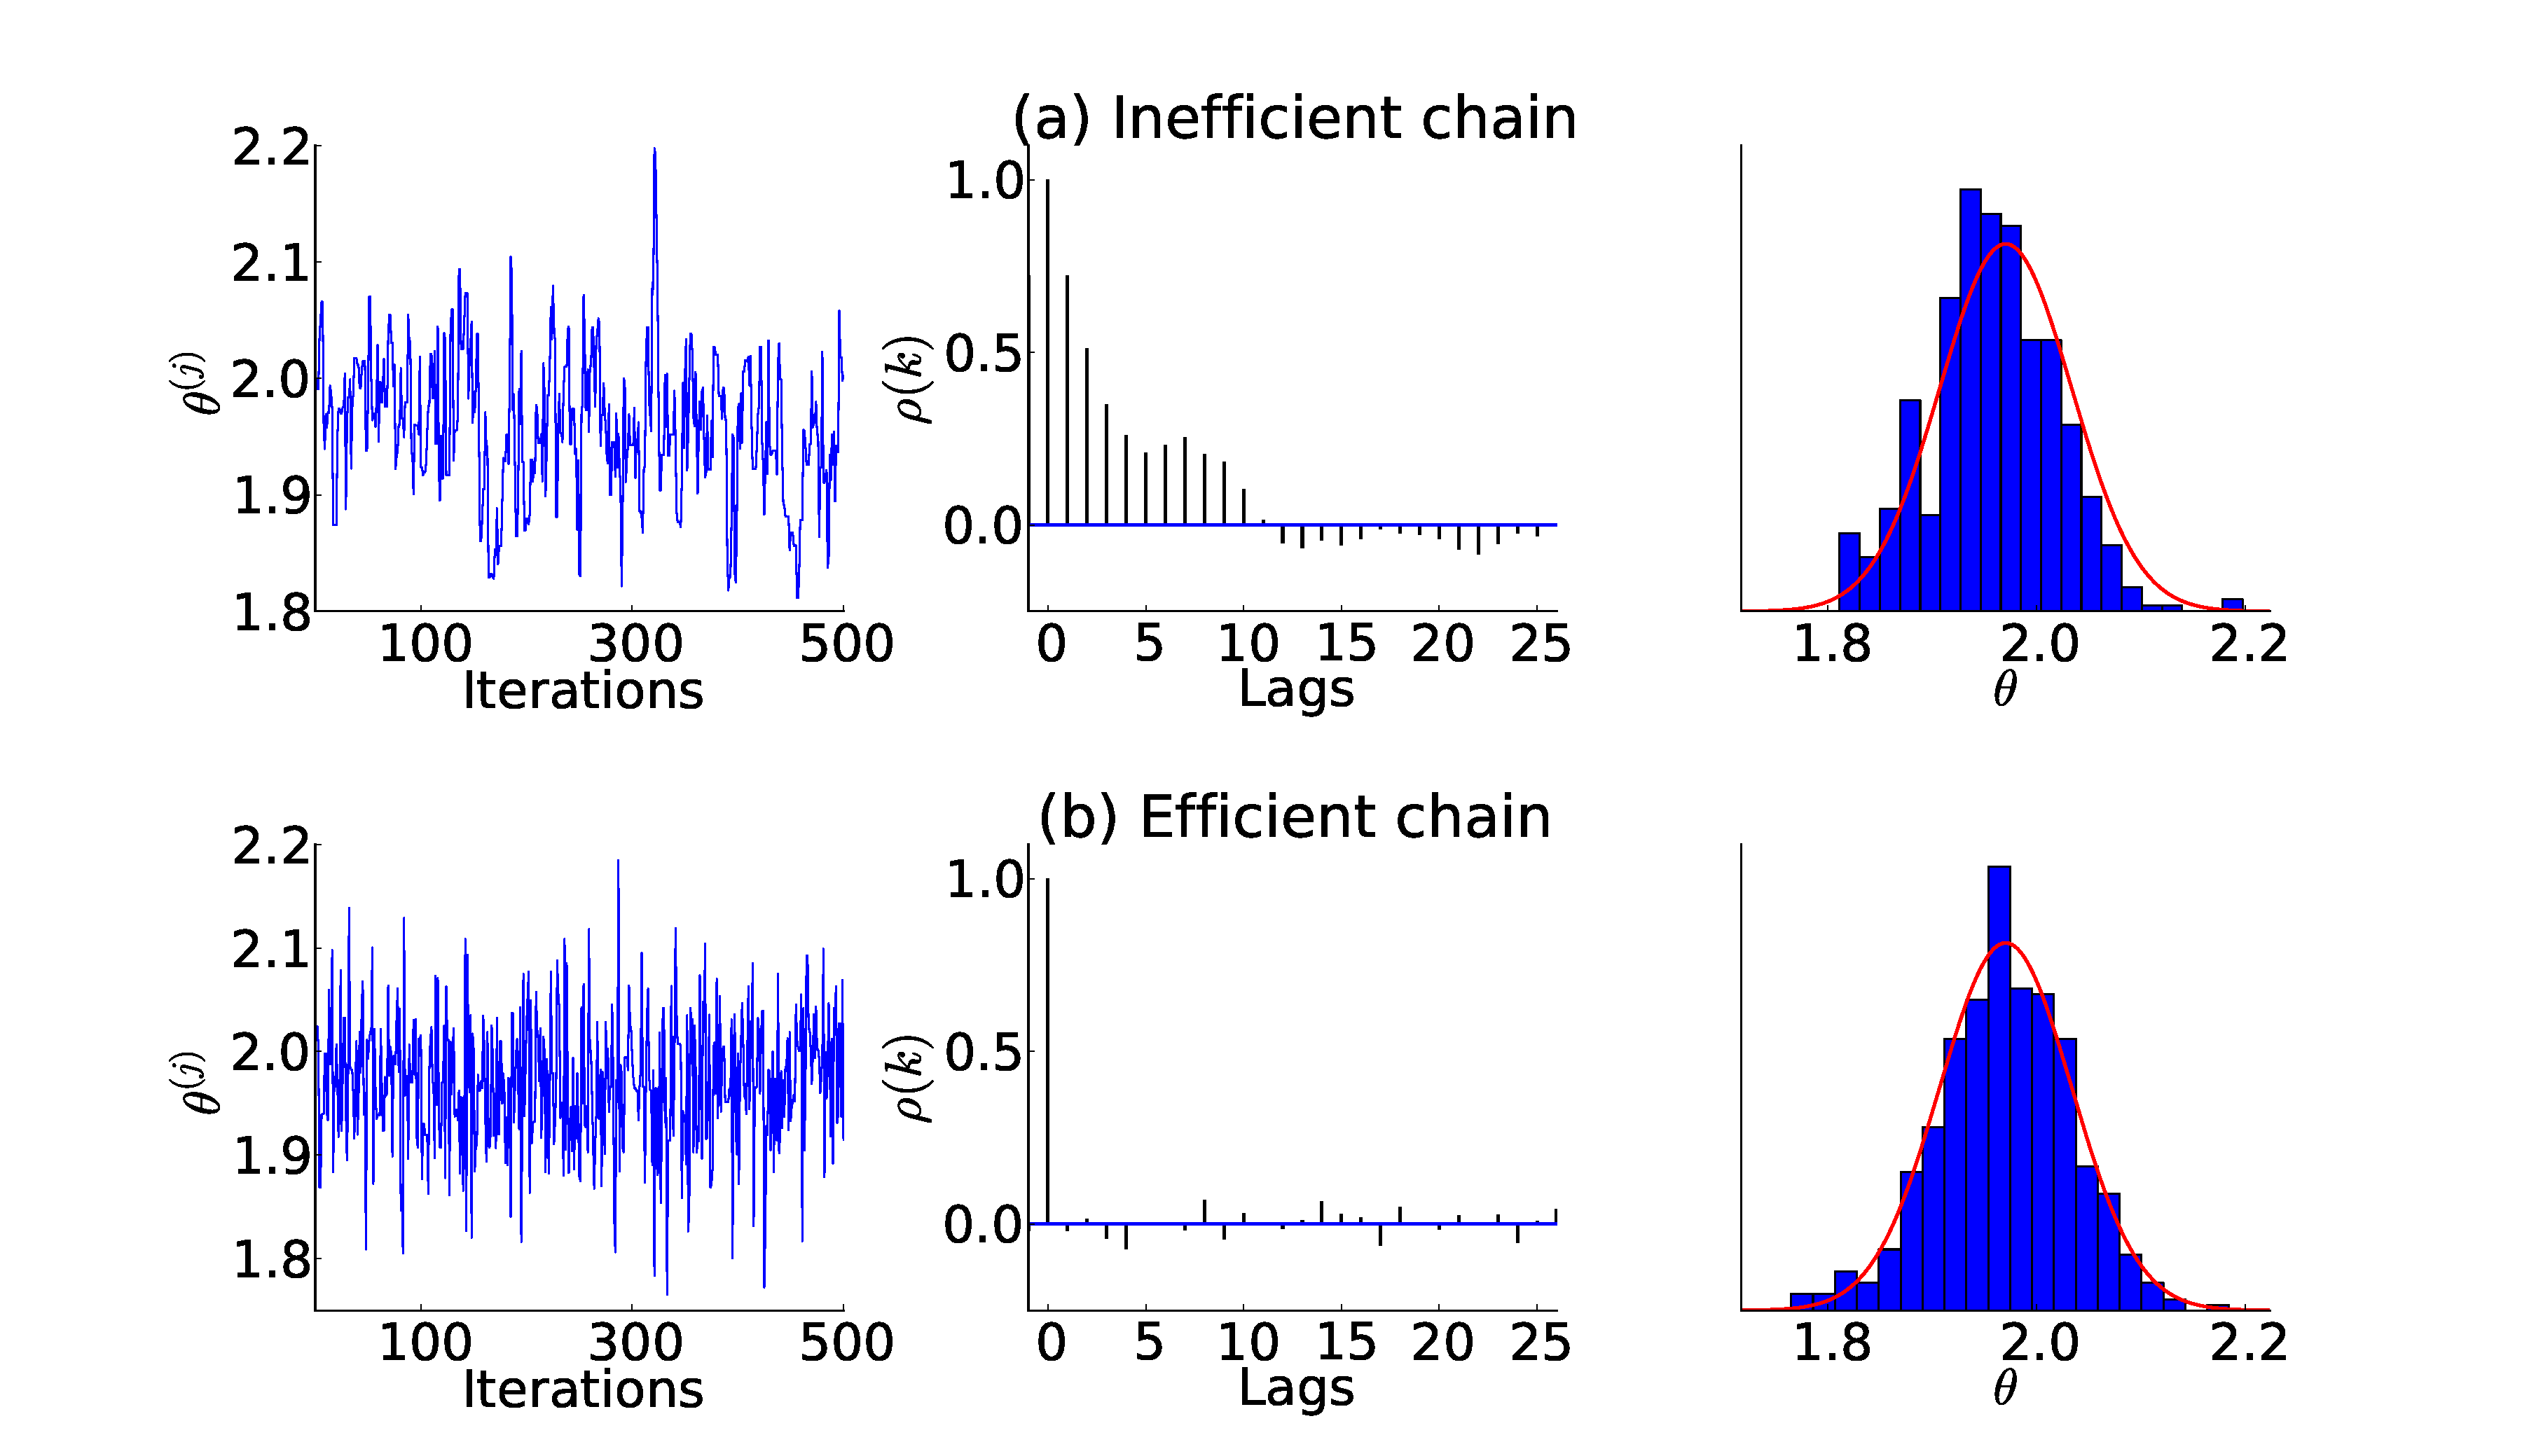
\includegraphics[width=1\columnwidth]{Efficiency}
\protect\caption{\textbf{\color{blue}Left:} trace plots of chain. \textbf{\color{blue}Middle:} auto-correlation of chain at lag $k$. \textbf{\color{blue}Right:} True posterior (red line) and MCMC approximation (histogram)}
\end{figure}
\end{frame}

\begin{frame}
\frametitle{Measures of efficiency - IF and ESS}
\begin{itemize}
\item With \textbf{\color{blue}MCMC}: The generated $\{\theta^{(i)}\}_{i=1}^N$ is a \textbf{\color{blue}dependent} sequence. 
\item How \textbf{efficient} is \textbf{MCMC} compared to \textbf{iid. sampling}?
\item \textbf{Variance of {\color{blue}posterior mean estimate}} if the \textbf{\color{red}sequence is iid}. 
$$V[\bar{\theta}]=Var\left[\frac{1}{N}\sum_{i=1}^N \theta^{(i)}\right]=\frac{\sigma^2}{N}\quad \left[\sigma^2 = V\left[\theta \right]\right].$$
\item \textbf{Variance of {\color{blue}posterior mean estimate}} if the \textbf{\color{red}sequence is dependent} % weakly stationary 
$$V[\bar{\theta}]=Var\left[\frac{1}{N}\sum_{i=1}^N \theta^{(i)}\right]=\frac{\sigma^2}{N}\times IF, \quad IF =\left(1 + 2 \sum_{k=1}^{\infty}\rho_k\right),$$
where $\rho_k = Corr(\theta^{(i)},\theta^{(i+k)})$ is the \textbf{\color{blue}auto-correlation} at lag $k$.
\end{itemize}
\end{frame}

\begin{frame}
\frametitle{Measures of efficiency - IF and ESS, cont.}
\begin{itemize}
\item IF is the \textbf{\color{blue}Inefficiency Factor} (IF) (or \textit{integrated auto-correlation time}): 
\\ The variance of the estimate \textbf{\color{red}inflates} $IF$ times for my MCMC (relative to iid. sampling).\bigskip
\item \textbf{\color{blue}Effective Sample Size} (ESS): $\textbf{ESS}=N/IF$.\bigskip
\item \textbf{Tells you}: how many \textbf{\color{red}equivalent to iid. draws} you get with your MCMC. \bigskip
\item Can be computed with the \texttt{CODA} package in \texttt{R} (Plummer et al., 2006). \textbf{\color{blue}Useful function}: \texttt{effectiveSize}.
\end{itemize}
\end{frame}


\begin{frame}
\frametitle{Improving the efficiency of MCMC}
\begin{itemize}
\item Most \textbf{\color{blue}essential} (but also the \textbf{most difficult}) find a \textbf{better proposal} $q$.
\item \textbf{\color{blue}Modify} your proposal. 
\\ For example in a \textbf{R-W Metropolis} make sure $\alpha \approx 0.23$. $$ \tilde{c}=\frac{2.4}{\sqrt{p}} \text{ gives [\textbf{in theory}] } \alpha \approx 0.23 \quad [p=\text{number of parameters}].$$
\\ \textbf{\color{red}Note}: only for a \textbf{R-W}. With \textbf{IMH} you want $\alpha$ as high as possible.
\item \textbf{\color{blue}Re-parametrization} helps a lot. \textbf{Especially} if the support of $\theta$ is \textbf{\color{red}restricted}.
\item \textbf{Example}
\begin{eqnarray*}
\text{if } \theta \in \mathbb{R}^{+} & \text{use} & \phi = \log(\theta) \\
\text{if } \theta \in [0,1] & \text{use} & \phi = \text{logit}(\theta),
\end{eqnarray*}
but (\textbf{again}!) \textbf{\color{red}do not forget the Jacobian}! [transformation of variables] 
\item Simple way to \textbf{reduce} auto-correlation: \textbf{\color{blue}thinning} - keep every $b$th sample.
\end{itemize}

\end{frame}

\begin{frame}
\frametitle{Assessing convergence of MCMC}
\begin{itemize}
\item \textbf{How long} is the \textbf{\color{blue}burn-in} period? 
\medskip
\item \textbf{\color{blue}Convergence diagnostics}:
\begin{itemize}
\item \textbf{Plot the Markov chains}. Do they seem to settle?
\item \textbf{Plot cumulative means}. Do the means converge?
\item Interested in a function $h(\theta)$? \textbf{Monitor its convergence}. 
\\ \textbf{\color{blue}Example:} 
\\ \textbf{Objective:} $h(\theta)=\Pr(\theta>2)$. \textbf{\color{blue}MCMC estimate} is $$\hat{I}_N = \{ \# \{\theta^{(i)}\}_{i=1}^N > 2\}/N \quad [\text{when \textbf{all} } N \text{ draws are available}].$$ Compute (and plot) $\hat{I}_k$ for $k=1,\dots,N$ and see if it converges.
\item \textbf{Do you suspect} your posterior is \textbf{multimodal}? Try different starting values.
\end{itemize}
\medskip
\item \textbf{\color{blue}Question}: How long to sample \textbf{after} the \textbf{\color{blue}burn-in} period?
\medskip
\item \textbf{\color{blue}Answer}: depends on IF (and ESS). An ESS of $1000$ is usually sufficient for most tasks.
\end{itemize}
\end{frame}


%\begin{frame}
%\frametitle{Time for some R coding!}
%\begin{itemize}
%\item \textbf{The script} \texttt{logitRWMH.R} revisits \textbf{logistic regression}: 
%\begin{itemize}
%\item Rewrites \texttt{logitRWMetropolis.R} to a \textbf{\color{blue}M-H} form (include proposal ratio).
%\item \textbf{Generalized} to $p$ parameters.
%\item \textbf{Computes} \textbf{\color{blue}IF} and \textbf{\color{blue}ESS} by \texttt{CODA}.
%\item \textbf{\color{blue}Posterior summary} and \textbf{\color{blue}posterior predictive simulation}.
%\end{itemize}
%\item Another R-script: \texttt{logitIMH.R} - implements the \textbf{Independence M-H}. The same thorough analysis as \texttt{logitRWMH.R}.
%\item \textbf{\color{blue}Homework:} Play with the codes.
%
%\end{itemize}
%\end{frame}


\begin{frame}
\frametitle{References}

\small{
\textbf{Chib, S. and Greenberg, E. (1995)}. Understanding the M-H algorithm. \textit{The American Statistician}, 49(4):327-335.}
\\~\\
\small{
\textbf{Plummer, M., Best, N., Cowles, K., and Vines, K. (2006)}. Coda: Convergence diagnosis and output analysis for MCMC, \textit{R News}, 6(1):7-11.
}

\end{frame}








\end{document}

